\makeatletter
\renewcommand\paragraph{\@startsection{paragraph}{4}{\z@}%
{-2.5ex\@plus -1ex \@minus -.25ex}%
{1.25ex \@plus .25ex}%
{\normalfont\normalsize\bfseries}}
\makeatother
\setcounter{secnumdepth}{5} % how many sectioning levels to assign numbers to
\setcounter{tocdepth}{5}
\makeindex

\begin {document}
\subsubsection{Servlets}
Die Tomcat-Servlets bilden zusammen einen Webservice in Anlehnung an einen \\
REST-Webservice (Representational State Transfer). \\
Im MVC-Paradigma würden sie in die Kategorie Controller fallen.\\
Die Servlets sind in verschiedene Aufgabenbereiche unterteilt. Alle Servlets \\erben von BaseServlet, was wiederum von HttpServlet erbt.
Die genaue Art der Anfrage wird über den QueryString der HttpServletRequest bestimmt.\\
Alle Anfragen werden in Form von JSON über die HTTP-POST methode übergeben.\\
In der doPost() Methode der Servlets werden sie bearbeitet.
die doGet() Methode wird bei einer HTTP-GET request aufgerufen. \\
Sie liefert Informationen
über den Zustand des Servlets, bzw. leitet den Nutzer weiter, falls er die Anfrage von einem Webbrowser aus sendet.\\
Über einen POST erhaltene Daten werden als JSON String interpretiert und via \\Jackson API auf Request-Objekte abgebildet.\\
Innerhalb des Request-Objekts sind Benutzer und Gruppen nur durch ID und Name spezifiziert.
Die zugehörigen Objekte werden aus der Datenbank angefordert. \\Name und ID dienen dabei als Schlüssel.\\
\\
Das GroupServlet als Beispiel zur server-internen Bearbeitung von Anfragen:
\\

\begin{figure}[h]
     \centering
     \hspace*{-2cm}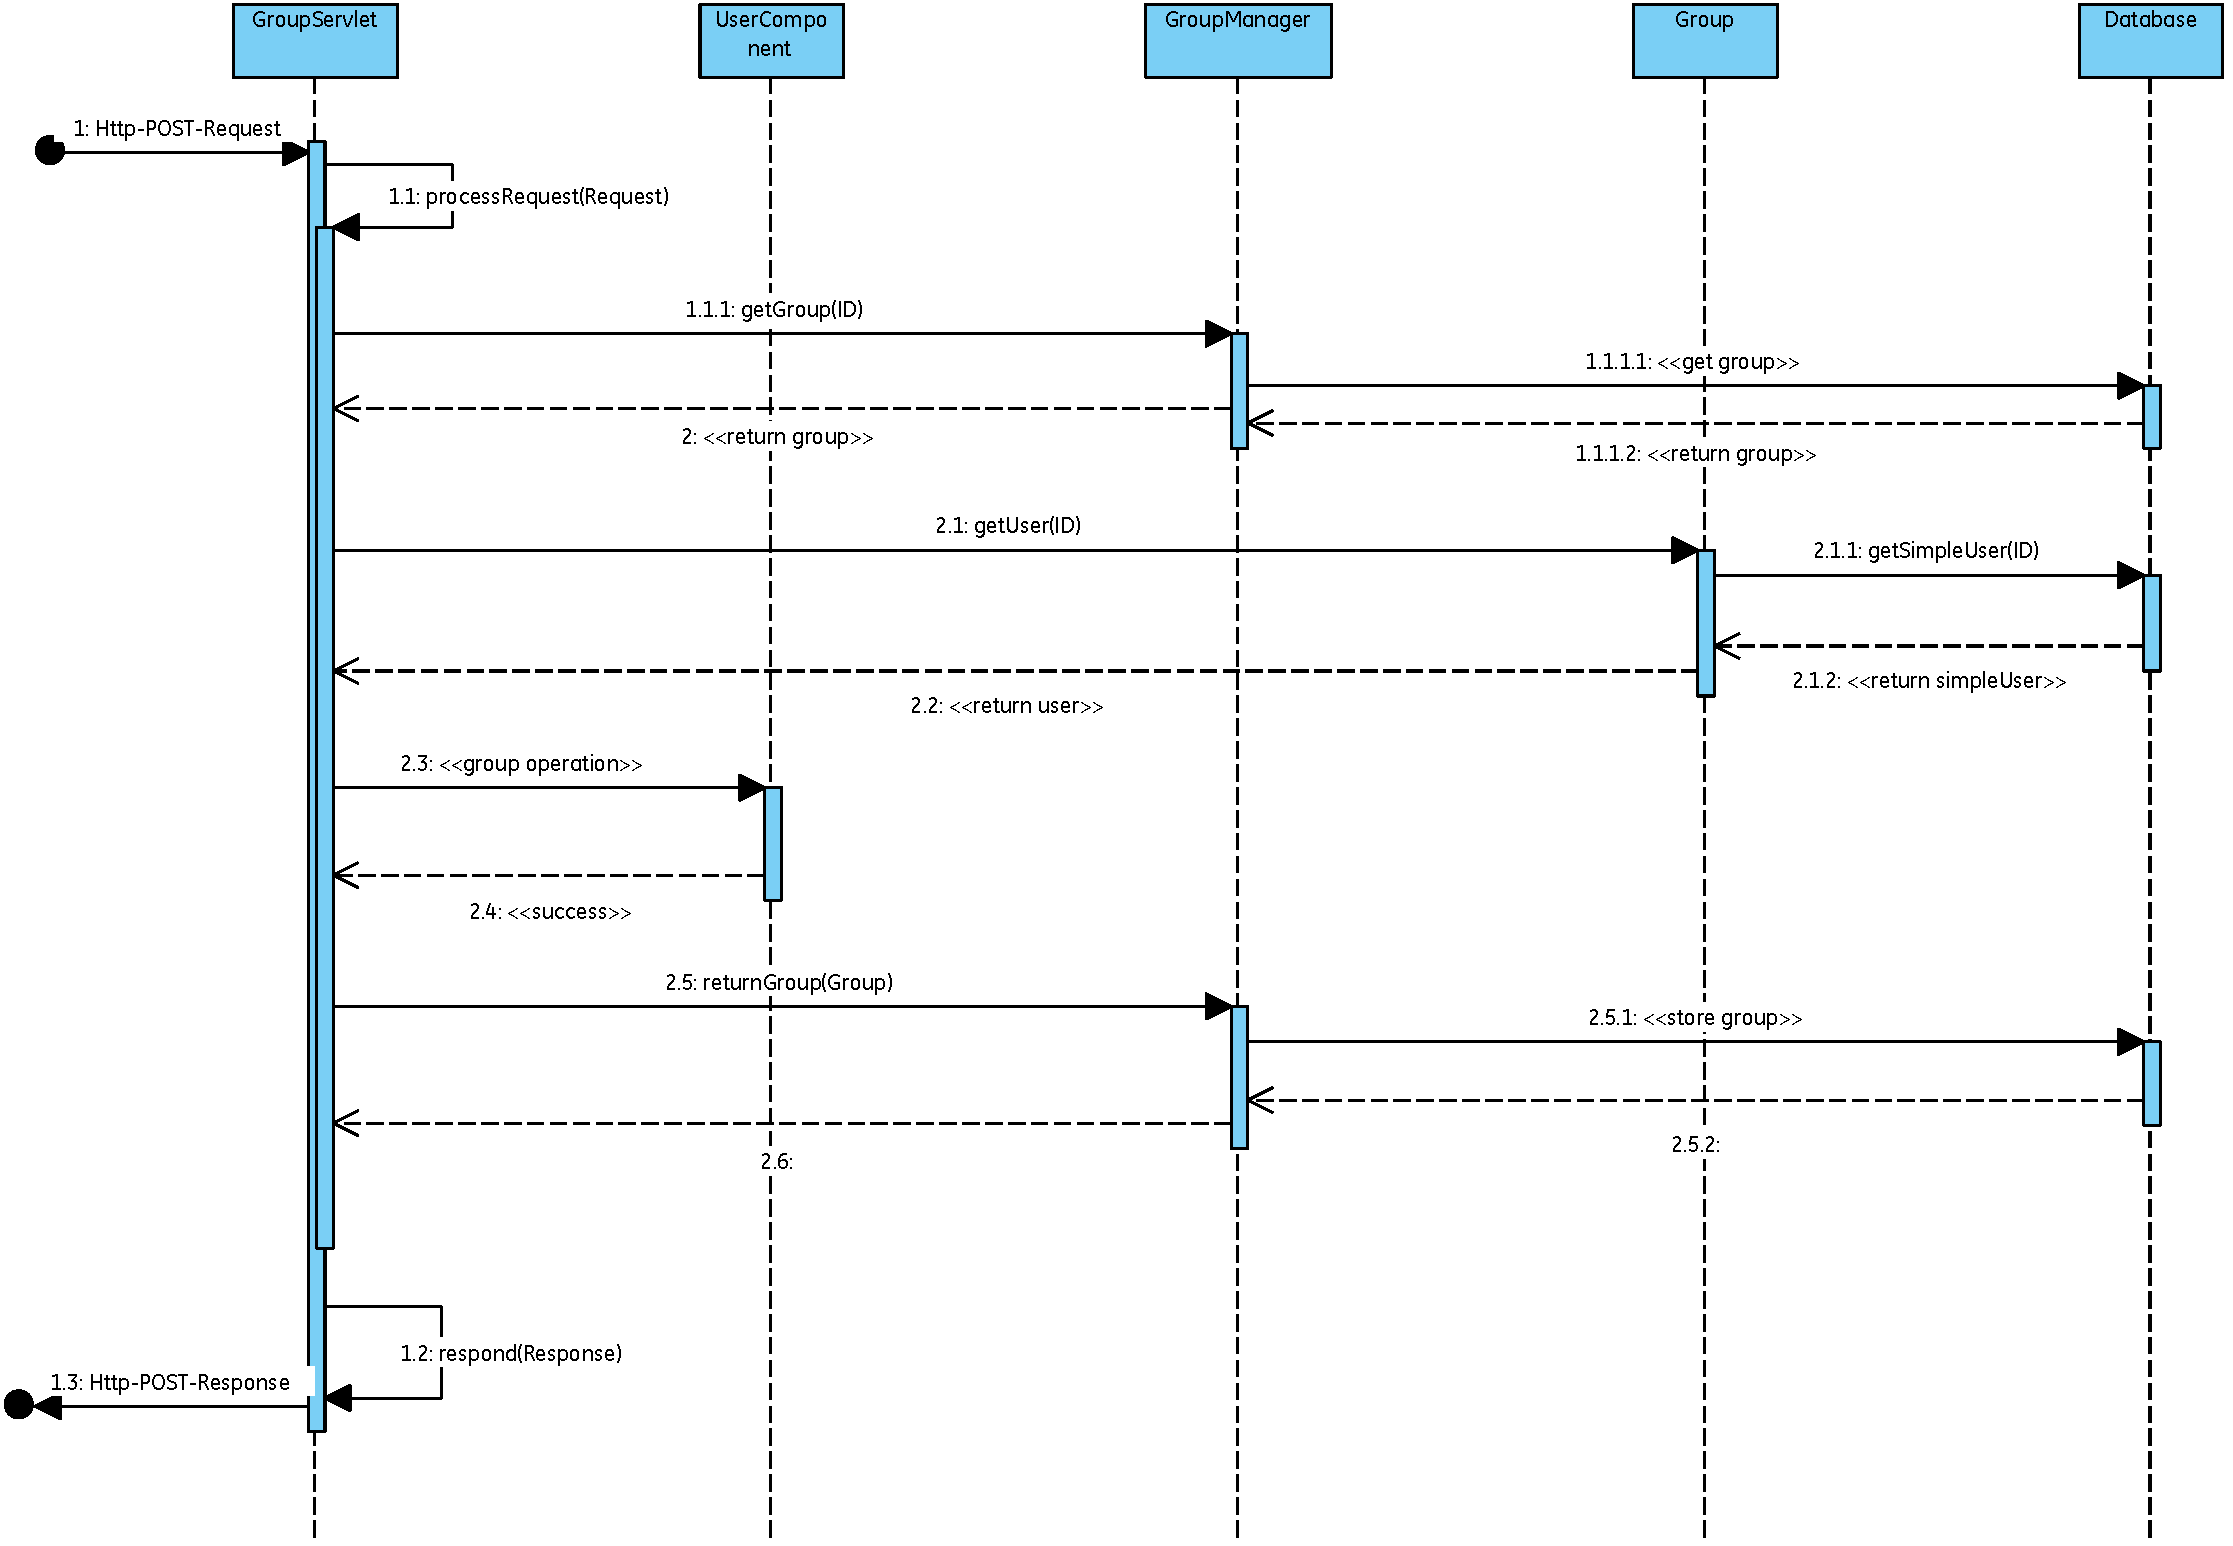
\includegraphics[scale=0.5, trim=2 2 2 2, clip=true]{servergraphs/sequenz-server.pdf}
     \caption{Sequenzdiagramm GroupServlet}
\end{figure}
\clearpage
\\
\begin{figure}[h]
     \centering
     \hspace*{-2.9cm}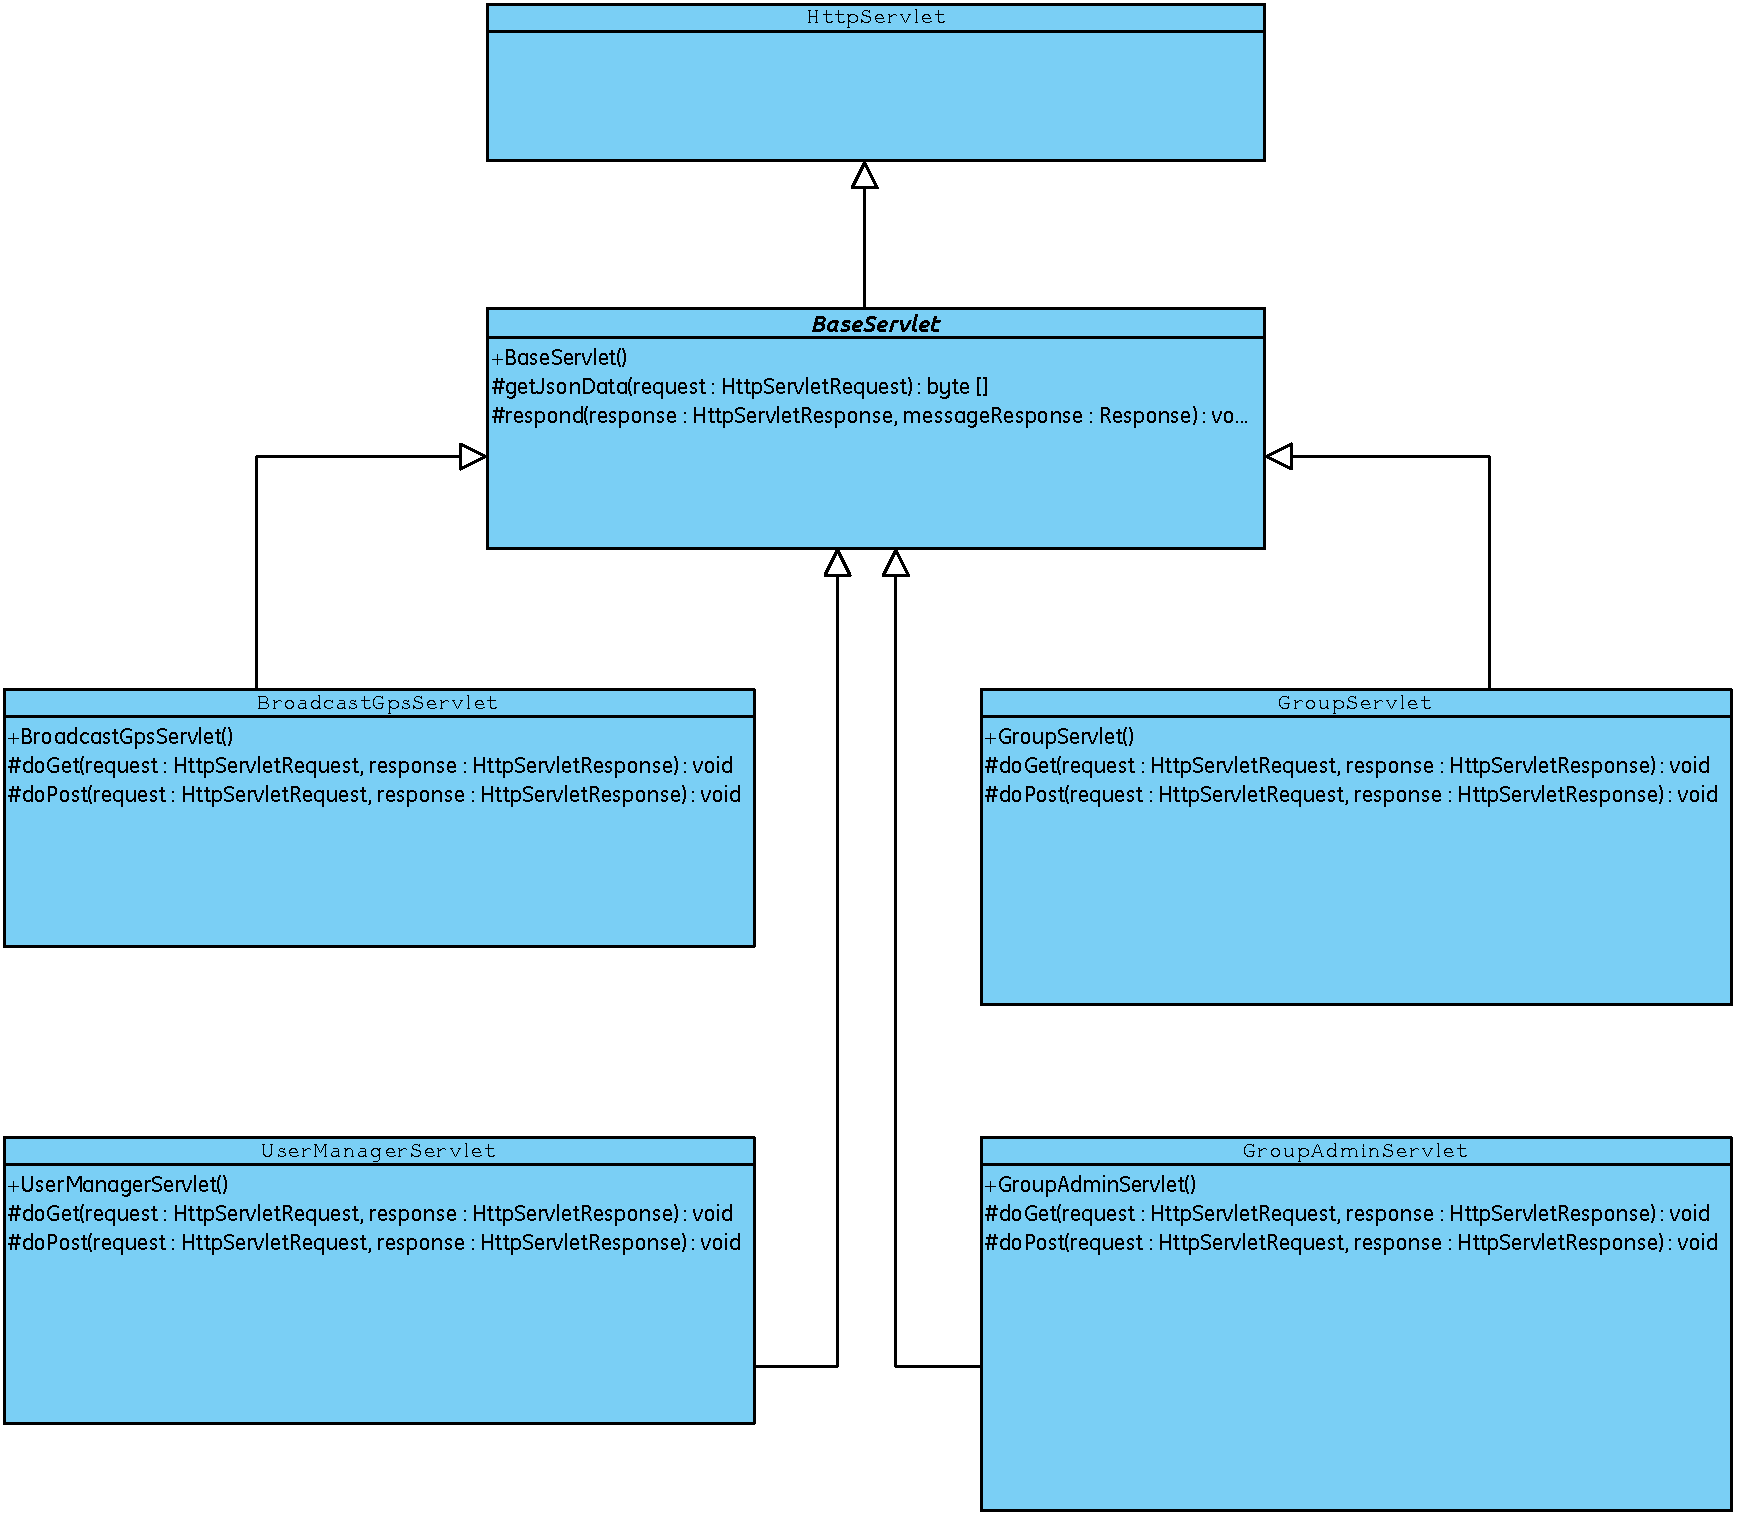
\includegraphics[scale=0.7]{servergraphs/servlets.pdf}
     \caption{Vererbungshierarchie der Servlets}
\end{figure}
\clearpage
\newpage
\textbf{Klasse GroupServlet} \\
\\
Zuständig für alle Nutzer-Anfragen bezüglich Gruppen. \\
Hier werden nur Parameter der Gruppe abgefragt. Administrative Anfragen werden vom GroupAdminServlet bearbeitet.\\
Von einem Gruppenmitglied abgefragt, werden beispielsweise aktueller Treffpunkt,\\
aktuelle Gruppenmitglieder oder aktueller Gruppenname.\\
Die GroupServlet Klasse dient als eine Schnittstelle zu der Datenbank auf dem Server.\\
Bildet die Anfrage auf ein GroupRequest Objekt ab.

\textbf{Klasse UserManagerServlet} \\
\\
Das UserManagerServlet ist für alle Benutzeroperationen zuständig. Dazu gehören:\\
Benutzeraccount anlegen, Benutzername ändern, Benutzer löschen.\\
Damit ist das UserManagerServlet eine weitere Schnittstelle zur Datenbank.\\
Bildet die Anfrage auf ein UserRequest Objekt ab.

\textbf{Klasse GroupAdminServlet} \\
\\
Im GroupAdminServlet werden alle Anfragen eines Gruppen-Administrators bearbeitet.\\
Dabei wird die Zielgruppe und der Nutzer in einem Request-Objekt übergeben.\\
Geprüft wird, ob der Benutzer Admin der Zielgruppe ist. Ist dies der Fall, \\
wird über den QueryString die gewünschte Operation auf der Gruppe ausgeführt.\\
Bildet die Anfrage auf ein GroupAdminRequest Objekt ab.

\textbf{Klasse BroadcastGpsServlet} \\
\\
In diesem Servlet werden von Gruppenmitgliedern gesendete GPS-Daten empfangen und in der
Datenbank gespeichert. Ist der GoStatus für ein Mitglied gesetzt,\\
können andere Mitglieder ihn Abrufen.\\
Bildet die Anfrage auf ein BroadcastGpsRequest Objekt ab.

\newpage
\subsubsection{Kommunikation}
Zum Datenaustausch zwischen Client und Server haben wir zwei Klassen erstellt:\\
Request und Response.\\
Davon erben die jeweils aufgabenspezifischen Request/Response-Klassen.\\
\\
\textbf{Klasse Request}\\
\\
Die abstrakte Request Klasse besteht hauptsächlich aus gettern und settern,\\
diese werden unter anderem von der Jackson API zum Serialisieren benötigt.\\
Dabei dient die Klasse ausschließlich als container und enthält keine Programmlogik.\\
Wichtig ist, dass nur ID's bzw. Namen in Form von String/Integer übergeben werden,\\
dadurch wird die Größe des resultierenden JSON-Strings möglichst klein gehalten.\\
\\ \\ \\

\begin{figure}[h]
     \centering
     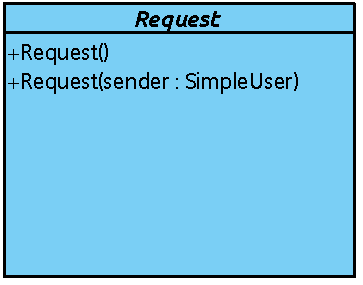
\includegraphics[scale=1.0,trim=2 2 2 2,clip=true]{servergraphs/request.pdf}
     \caption{Klassendiagramm Request}
\end{figure}
\clearpage

\begin{figure}[h]
\hspace*{-1.8cm}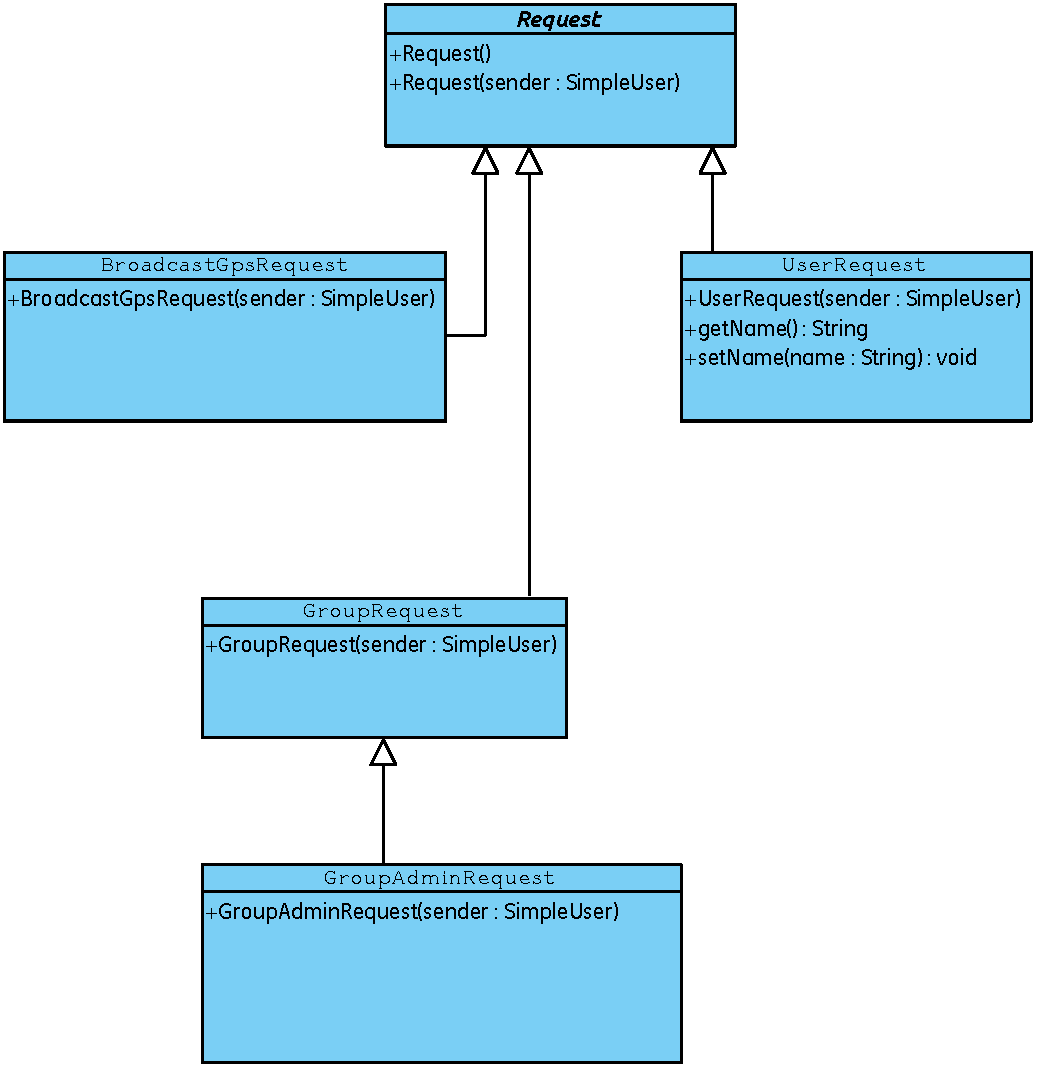
\includegraphics[scale=1.0,trim=2 2 2 2,clip=true]{servergraphs/communication-request.pdf}
     \caption{Vererbungshierarchie Request}
\end{figure}
\clearpage

\textbf{Klasse UserRequest}\\
\\
UserRequest ist eine Anfrage um einen neuen Benutzeraccount anzulegen, \\
bzw. falls schon vorhanden, den Benutzernamen zu ändern.\\

\textbf{Klasse GroupRequest}\\
\\
Alle gruppenbezogenen Anfragen. Benötigt werden Benutzer-ID, Name der entsprechenden
Gruppe, und ein QueryString, der die Operation beschreibt, die auf der Gruppe\\
ausgeführt werden soll.\\
Dieser Anfragetyp kann nur von einem Gruppenmitglied gesendet werden.\\
Diese Anfrage kann gesendet werden um den aktuellen Stand einer Gruppe abzufragen.\\
Änderungen sind zum Beispiel wenn ein neuer Treffpunkt gesetzt wurde, \\
ein Benutzer der Gruppe beigetreten ist, oder ein Benutzer die Gruppe verlassen hat.\\

\textbf{Klasse GroupAdminRequest}\\
\\
GroupAdminRequest ist eine erweiterung der normalen GroupRequest. Sie enthält\\
zusätzlich alle Anfragen eines Gruppenadministrators. Dazu zählen: Gruppe löschen,\\
Gruppe umbenennen, Mitglieder einladen, etc.\\
Die Klasse hält die Variablen für jede mögliche Administrator-Anfrage.\\

\textbf{Klasse BroadcastGpsRequest}\\
\\
Anfrage um die eigenen GPS-Daten an die Gruppe zu verteilen, oder GPS-Daten der\\
anderen Gruppenmitglieder abzufragen.\\
Die eigenen GPS-Daten sind nicht zwingend notwendig, da das anfragende Mitglied seinen\\
Status auf 'Go' setzen kann, ohne die eigenen GPS-Daten preiszugeben.\\

\newpage
\textbf{Klasse Response}\\
\\
Als Antwort auf eine Request sendet der Server eine Response an den Client.\\
Die Response enthält alle angeforderten Daten bzw. manipulierte Daten und \\
ob die Operation, die der Nutzer angefragt hat, erfolgreich war.\\
Auf einfache Anfragen, wie beispielsweise den eigenen Benutzernamen zu ändern,\\
wird mit einer einfachen Response geantwortet, die dem Nutzer sagt,\\
ob der Name erfolgreich geändert wurde.\\
\\ \\ \\ \\

\begin{figure}[h]
     \hspace*{-2cm}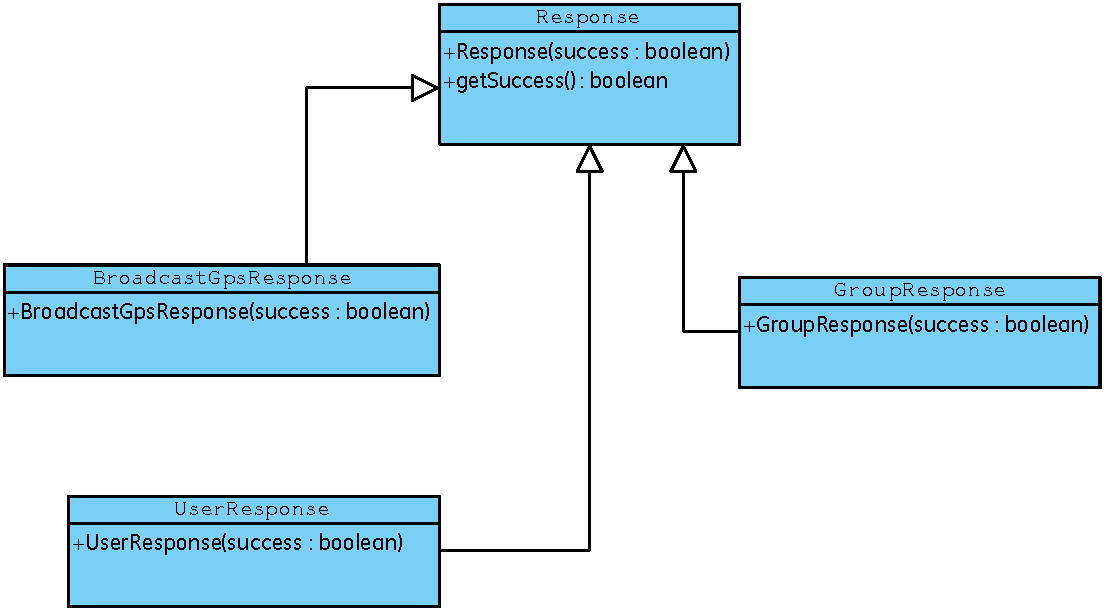
\includegraphics[scale=1.0]{servergraphs/communication-response.pdf}
     \caption{Vererbungshierarchie Response}
\end{figure}
\clearpage

\textbf{Klasse UserResponse}\\
\\
Anwort auf eine Nutzername ändern Anfrage oder eine Registrieren Anfrage.\\
Bei der Registrierung wird eine eindeutige Benutzer-ID zurückgegeben.\\
Im Falle einer Benutzername-ändern-Anfrage wird nur der Status zurückgegeben.\\

\textbf{Klasse GroupResponse}\\
\\
Antwort auf eine Gruppen-Anfrage oder eine Administrator-Anfrage.\\
Ein GroupResponse-Objekt enthält dabei die, nach der Operation, aktuelle Gruppe.\\
Bei einer Update-Anfrage wird ebenfalls mir einer GroupResponse geantwortet.\\

\textbf{Klasse BroadcastGpsResponse}\\
\\
Als Antwort auf eine BroadcastGpsRequest, enthält die BroadcastGpsResponse die GPS-Daten\\
der anderen Gruppenmitglieder, die bereits 'Go' gedrückt haben, also ihre Daten bereits\\
an den Server gesendet haben.\\
\newpage

\subsubsection{Server-Modell}
Das Modell des Servers unterscheidet sich in wesentlichen Punkten zu dem des Clients:\\
Operationen auf Gruppen oder Benutzern lösen keine Anfragen an einen Server aus,\\
sondern arbeiten direkt mit der Schnittstelle zur Datenbank.\\
Das Client-Modell stellt praktisch die 'Fernbedienung' für das Server-Modell dar.\\
\\
\textbf{Hibernate}\\
\\
Die Schnittstelle unserer Datenbank stellt Hibernate dar. Dazu werden in den Klassen
GroupAdminServer, GroupMemberServer und SimpleUser (Also alles was gespeichert werden muss), Annotations gesetzt, die Hibernate zum Abbilden benötigt.
Anfragen an die Datenbank werden von GroupManager und UserManager gesteuert.\\
\\
\textbf{Klasse UserManager}\\
\\
Der UserManager verwaltet Benutzeraccounts und bietet eine allgemeine Schnittstelle\\
zur Datenbank. Er hat zwei Methoden um ein Benutzer-Objekt aus der Datenbank\\
anzufordern: getUserById(int ID) - durchsucht die Datenbank nach einem User mit\\
gegebener Nutzer-ID und getUserByDevId(String devID) - durchsucht die Datenbank\\
nach einem Benutzer mit passender Geräte-ID. \\
Darüber werden die meisten Benutzer identifiziert, die eine Anfrage senden.\\
Die Nutzer-ID ist dazu gedacht, dass Gruppenmitglieder nicht die Geräte-ID der \\
anderen Mitglieder erfahren.\\
createUser(String Name) - Erzeugt einen Neuen Benutzer mit gegebenem Namen.\\
deleteUser(String devId) - Löscht den Benutzer mit der gegebenen Geräte-ID.\\
\\ \\ \\

\begin{figure}[h]
     \centering
     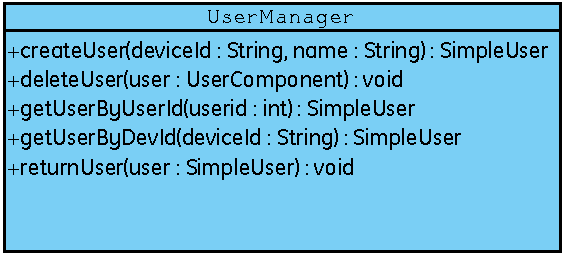
\includegraphics[scale=1.0, trim=1 1 1 1,clip=true]{servergraphs/user-manager.pdf}
     \caption{Klassendiagramm UserManager}
\end{figure}
\clearpage

\textbf{Klasse GroupManager}\\
\\
Gleichermaßen wir der UserManager, bietet auch der GroupManager eine \\
Schnittstelle zur Datenbank. Er bietet die Fabrikmethode createGroup()\\
zum Erstellen neuer Gruppen. Die Methode legt dazu einen neuen Eintrag in der\\
Datenbank an und liefert das neue Group-Objekt zurück.\\

\\ \\ \\
\begin{figure}[h]
     \centering
     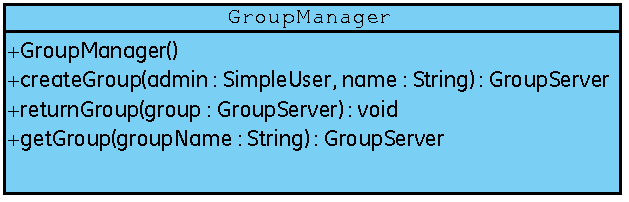
\includegraphics[scale=1.0, trim=2 2 2 2, clip=true]{servergraphs/group-manager.pdf}
     \caption{Klassendiagramm GroupManager}
\end{figure}
\clearpage

\textbf{Klasse GroupServer}\\
\\
Serverseitige Darstellung einer Gruppe. Operationen werden auf der Gruppe nicht\\
direkt ausgeführt. Nach dem Erstellen der Gruppe, laufen alle Operationen über den\\
Gruppenadministrator. über getMember(ID) bekommt man das Mitglied, dass man in \\
der aktuellen Gruppe darstellt. Also entweder GroupMember oder GroupAdmin.
In der Fabrikmethode getMember(ID) wird dem UserDecoratorServer das Gruppen-Objekt\\
übergeben, an dass dieser dann gebunden ist.\\

\\
\begin{figure}[h]
     \centering
     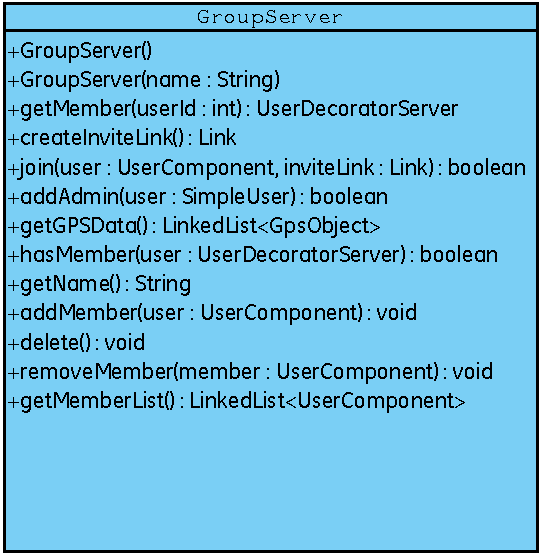
\includegraphics[scale=1.0, trim=2 2 2 2, clip=true]{servergraphs/group-server.pdf}
     \caption{Klassendiagramm GroupServer}
\end{figure}
\clearpage

\textbf{Klasse LinkGenerator}\\
\\
Die Aufgabe des LinkGenerators besteht darin, zu einer gegebenen Gruppe einen \\
Einladungslink zu generieren. Dabei wird an die Basis-URL des GroupServlets der\\
Gruppenname und ein zufällig generierter String angehängt.\\

\\
\begin{figure}[h]
     \centering
     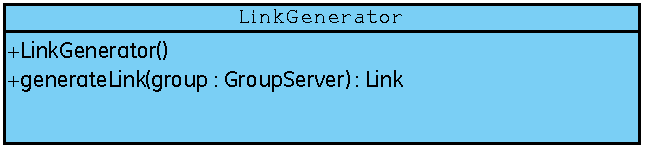
\includegraphics[scale=1.0, trim=2 2 2 2, clip=true]{servergraphs/link-generator.pdf}
     \caption{Klassendiagramm LinkGenerator}
\end{figure}
\clearpage

\textbf{Klasse Link}\\
\\
Da die Klasse Link aus dem common package für Client bereits dokumentiert ist,\\
sind hier nur noch ein paar Anmerkungen.
Ein Link vom Administrator einer Gruppe erzeugt und ist an die Gruppe gebunden.\\
Diese Klasse repräsentiert eine Gruppeneinladung. über die Getter kann man unabhängig\\
den Gruppennamen und das Geheimnis abfragen.\\
Hat man als Administrator den Link vom Server erhalten, wird über die toString() \\
Methode die endgültige URL erstellt. Diese kann nun über andere Wege versendet werden.
Öffnet man eine zugesendete URL mit der GoApp, wird daraus eine GroupRequest erzeugt,
mit der ein anderer Nutzer der Gruppe beitreten kann.\\
Das Geheimnis wird im zugehörigen Gruppen-Objekt gespeichert.\\
\\ \\ \\
\begin{figure}[h]
     \centering
     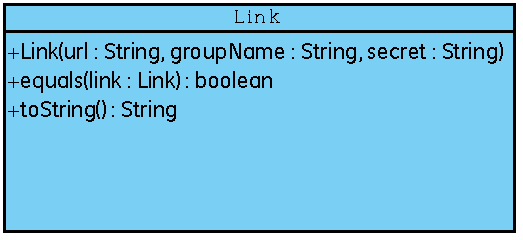
\includegraphics[scale=1.0, trim=2 2 2 2, clip=true]{servergraphs/link.pdf}
     \caption{Klassendiagramm LinkGenerator}
\end{figure}
\clearpage

\newpage
\textbf{Klasse UserDecoratorServer}\\
\\
Das serverseitige Gegenstück zum UserDecorator. Er implementiert das gleiche Interface
wie der UserDecorator auf dem Client, nur dass er mit GroupServer arbeitet. \\
Im UserDecoratorServer sind sowohl die Methoden des Admins, wie auch die des\\
einfachen GroupMembers vorhanden. Die Idee dahinter ist, dass man nicht verhindern\\
kann, dass ein normaler GroupMember eine Admin-Anfrage sendet.\\
Die Implementierung der beiden Klassen unterscheidet dann das Verhalten.\\
(Siehe GroupAdminServer und GroupMemberServer)\\

\\ \\ \\
\begin{figure}[h]
     \centering
     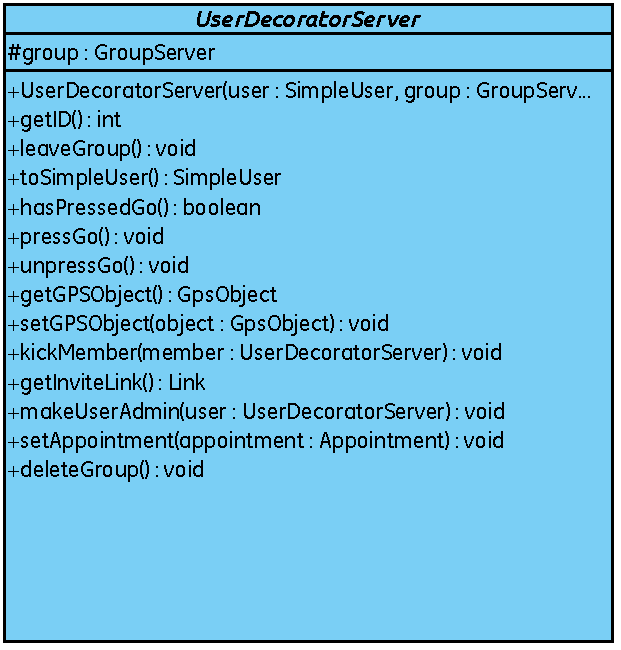
\includegraphics[scale=0.9]{servergraphs/user-decorator-server.pdf}
     \caption{Klassendiagramm UserDecoratorServer}
\end{figure}
\clearpage

\begin{figure}[h]
     \centering
     \hspace*{-2.6cm}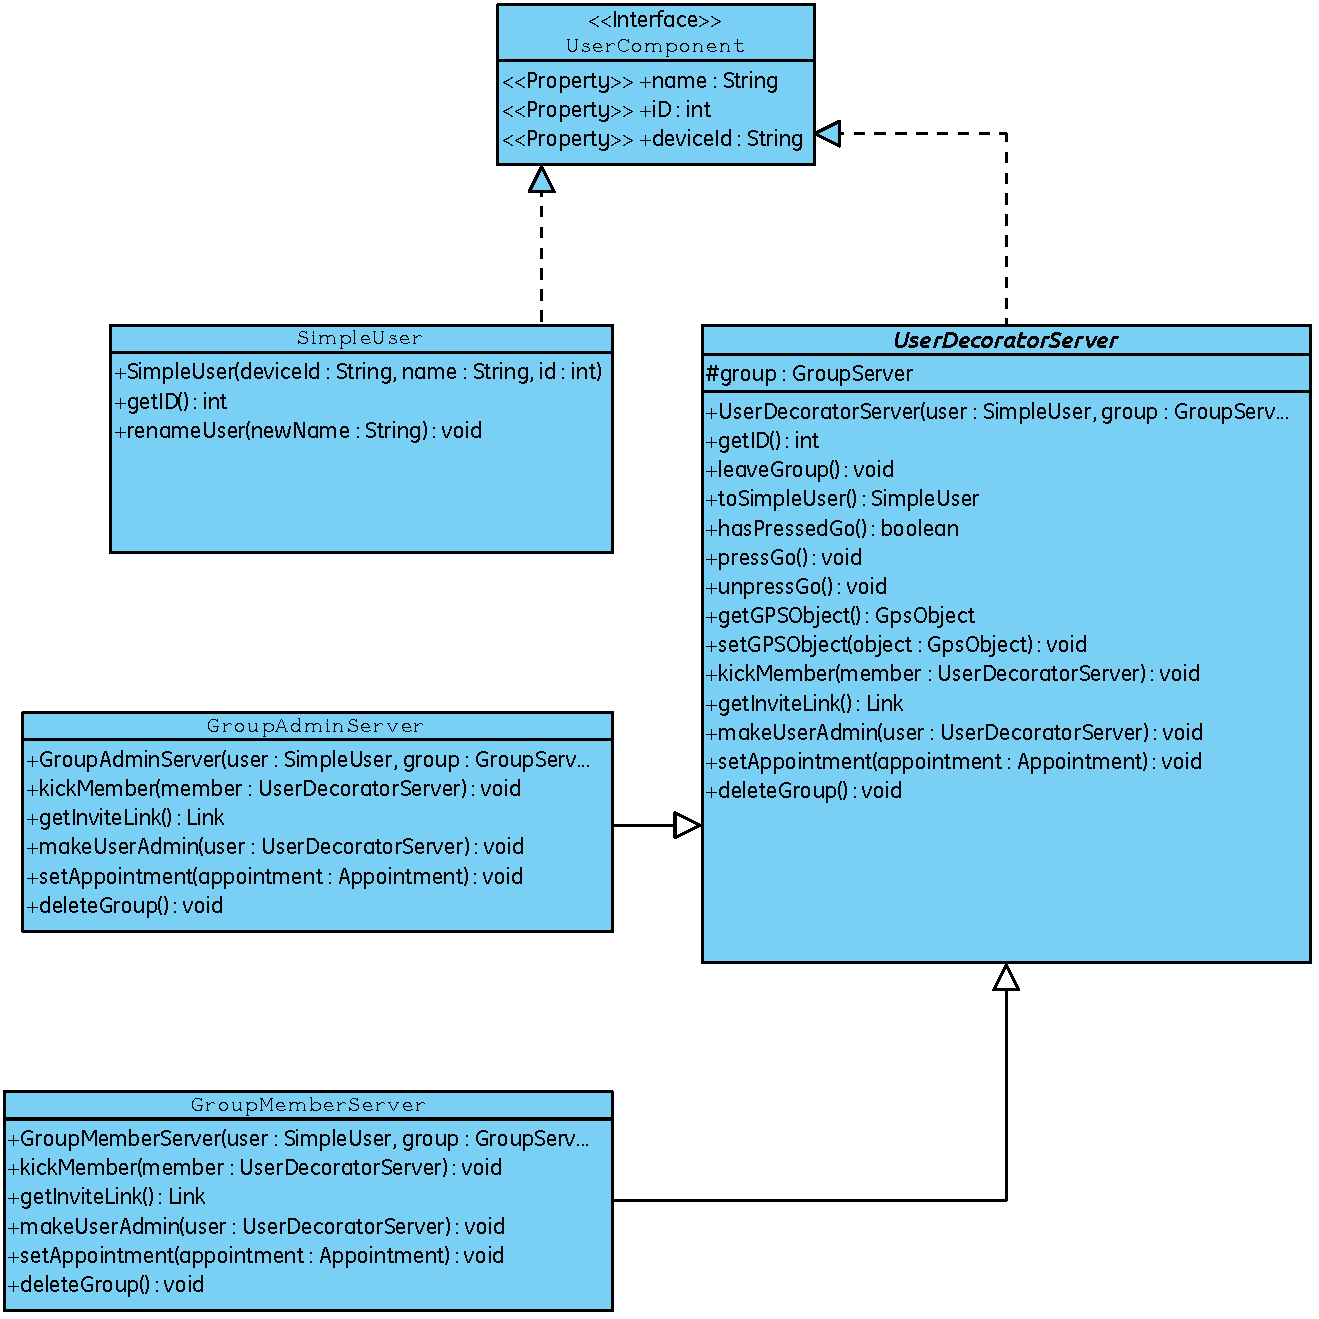
\includegraphics[scale=0.9]{servergraphs/user-component.pdf}
     \caption{Klassenhierarchie UserDecoratorServer}
\end{figure}
\clearpage

\textbf{Klasse GroupMemberServer}\\
\\
Die serverseitige Klasse für Gruppenmitglieder. Die einfache Implementierung eines\\
Gruppenmitglieds ohne besondere Rechte.\\
Die Klasse GroupMemberServer implementiert auch die Methoden des Administrators,\\
falls ein skrupelloses Gruppenmitglied eine Admin-Anfrage sendet, wird dabei\\
jedoch eine Fehlermeldung ausgelöst.\\

\textbf{Klasse GroupAdminServer}\\
\\
Die Gruppen-Administrator Klasse auf dem Server steuert alle Gruppenoperationen,\\
das heißt, wenn man über group.getUser(ID) ein Objekt der Klasse GroupAdminServer\\
zurückbekommt, kann man darüber die Gruppe 'group' kontrollieren.\\
Als Indirektion ruft der
Die Operationen sind an die Gruppe gebunden, auf der man getUser(ID) aufruft.\\

\end {document}
